\pagenumbering{arabic}

\chapter{Hey}
\section{Bruh}
This thesis is an exposition of two topics in the theory of 
algebraic plane curves, the theory of intersection multiplicities 
and the famous Theorem of Bezout.  In addition, we also look at
the special case of curves of degree three (the \emph{cubic}
curves) and explore some interesting properties of cubics.


Our main references are \cite{ST}, \cite{bix}, \cite{fulton}, 
and \cite{gibson}.  Other good books on algebraic curves are
\cite{kirwan} and \cite{walker}.

\section{A few Lemmas}
We begin with a table of the first few prime numbers.
This illustrates how to do tables.  We use the following commands

\begin{verbatim}
\begin{table}
\begin{center}\fbox{Such a table should appear here}\end{center}
\caption{The first 100 prime numbers}
\end{table}
\end{verbatim}

\begin{table}
\begin{center}\fbox{Such a table should appear here}\end{center}
\caption{The first 100 prime numbers}
\end{table}

\section{Some more stuff}

\chapter{I Can Write A Chapter Here?}
\section{The Main Result}
In this section, we show a picture of an elliptic curve,
thus illustrating how to do figures.

\begin{figure} 
\centerline{ 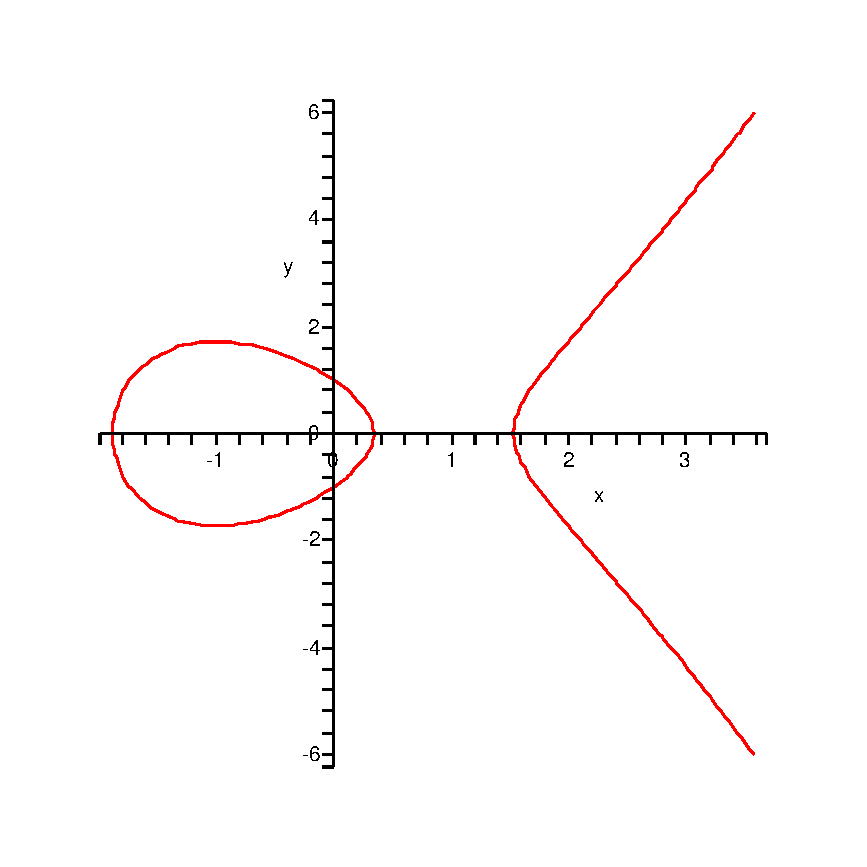
\includegraphics[width=4in]{elliptic.eps} }
\caption{An elliptic cubic}
\end{figure}

\begin{verbatim}
\begin{figure} 
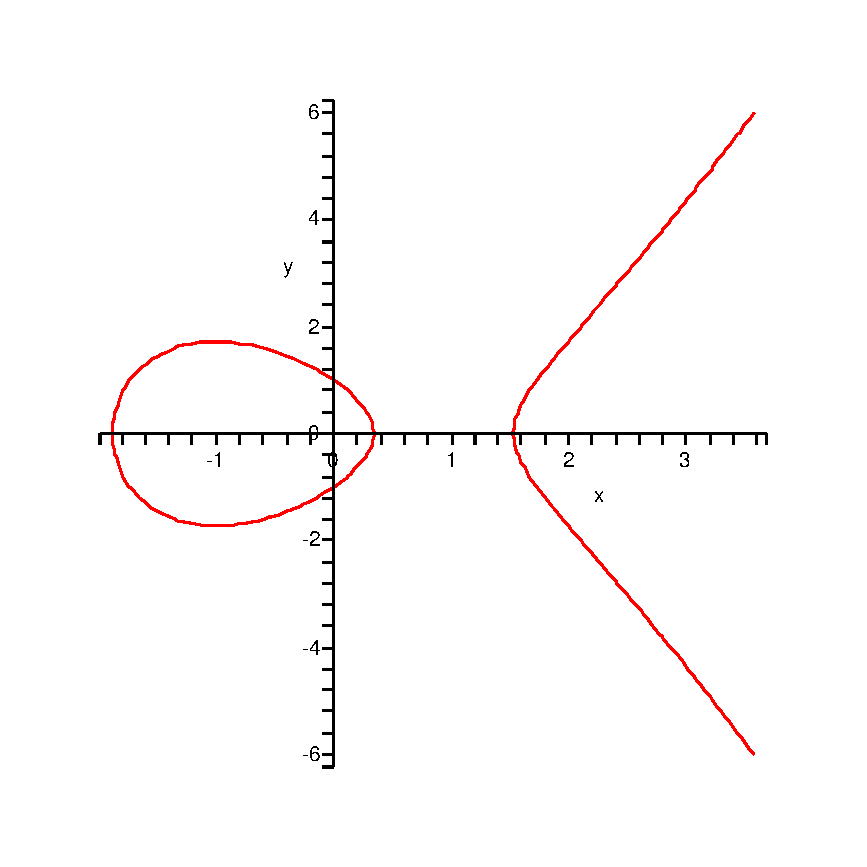
\includegraphics{elliptic}
\caption{An elliptic curve}
\end{figure}
\end{verbatim}

\section{Generalizations}


